% Max Smolens
% max@cs.unc.edu

\documentclass[11pt,letterpaper]{article}

\usepackage{fullpage, setspace}
\usepackage[numbers]{natbib}
\usepackage{graphicx}
\usepackage{url}

\author{Max Smolens\\ max@cs.unc.edu}
\date{\today}
\title{Bayer Pattern Renderer}

\begin{document}

\maketitle
\section{Introduction}
%\doublespace

Digital imaging devices that use CCDs commonly use a Bayer
pattern~\cite{bayer_patent} color filter array (CFA).  Because only
one color component is available at each position of the CFA, the two
missing color components at each position must be interpolated from
the available data.  This document describes the operation of a Bayer
pattern renderer that uses OpenGL to perform bilinear interpolation of
the Bayer pattern to generate a complete RGB image.
\section{Bayer Pattern}

The Bayer pattern consists of a repeated two-by-two color pattern that
consists of one red component, one blue component, and two green
components, as shown in Figure~\ref{fig:bayer_pattern}.

\begin{figure}
\centering
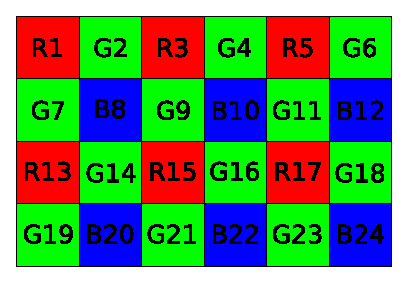
\includegraphics{bayer_pattern}
\caption{Bayer pattern.}
\label{fig:bayer_pattern}
\end{figure}
\section{Bilinear Interpolation of the Bayer Pattern}

A Bayer pattern image contains only one color component at each pixel.
Interpolation uses the available components from neighboring pixels to
fill in the two missing components at each pixel.  Bilinear
interpolation is relatively simple and fast compared to other
interpolation techniques available~\cite{tingchen}.  Pixels at the edge
of the image might need to be handled specially.
\subsection{Interpolating Green Components}

The green component for red and blue pixels in a Bayer pattern image
is the average of the four neighboring green pixels.  For example, in
Figure~\ref{fig:bayer_pattern}, \(G8\gets(G2+G7+G9+G14)/4\).
\subsection{Interpolating Red and Blue Components}

At a green pixel in a Bayer pattern image, the red component is the
average of the two adjacent red pixels.  For example,
\(R2\gets(R1+R3)/2\), and \(R9\gets(R3+R15)/2\).  The blue
components are calculated similarly.  For example,
\(B9\gets(B8+B10)/2\), and \(B16\gets(B10+B22)/2\).

At red and blue pixels in a Bayer pattern image, the missing red or
blue component is the average of the four diagonally-neighboring
pixels.  For example, \(R8\gets(R1+R3+R13+R15)/4\), and
\(B15\gets(B8+B10+B20+B22)/4\).
\section{Bilinear Interpolation of the Bayer Pattern Using OpenGL}

OpenGL's texture mapping functions can be used to approximate the
bilinear interpolation of the Bayer pattern to give the complete RGB
image.  The \texttt{BayerRenderer} class uses the render-to-texture
functions provided by the \texttt{RenderTexture}
class~\cite{rendertexture}.
\subsection{Color Channel Extraction}

The Bayer image is first loaded into texture memory.  The four color
channels in the Bayer image --- red, blue, and two greens --- are each
extracted into their own textures.  By setting the Bayer pattern
texture's minification function to \texttt{GL\_NEAREST} and applying a
different pixel offset to the texture matrix stack for each channel,
the individual channels are extracted into their own textures, as
shown in Figure~\ref{fig:channel_extraction}.  Because each of these
textures holds a quarter of the Bayer pattern image data, each is a
quarter of the size of the Bayer pattern texture.

\begin{figure}
\centering
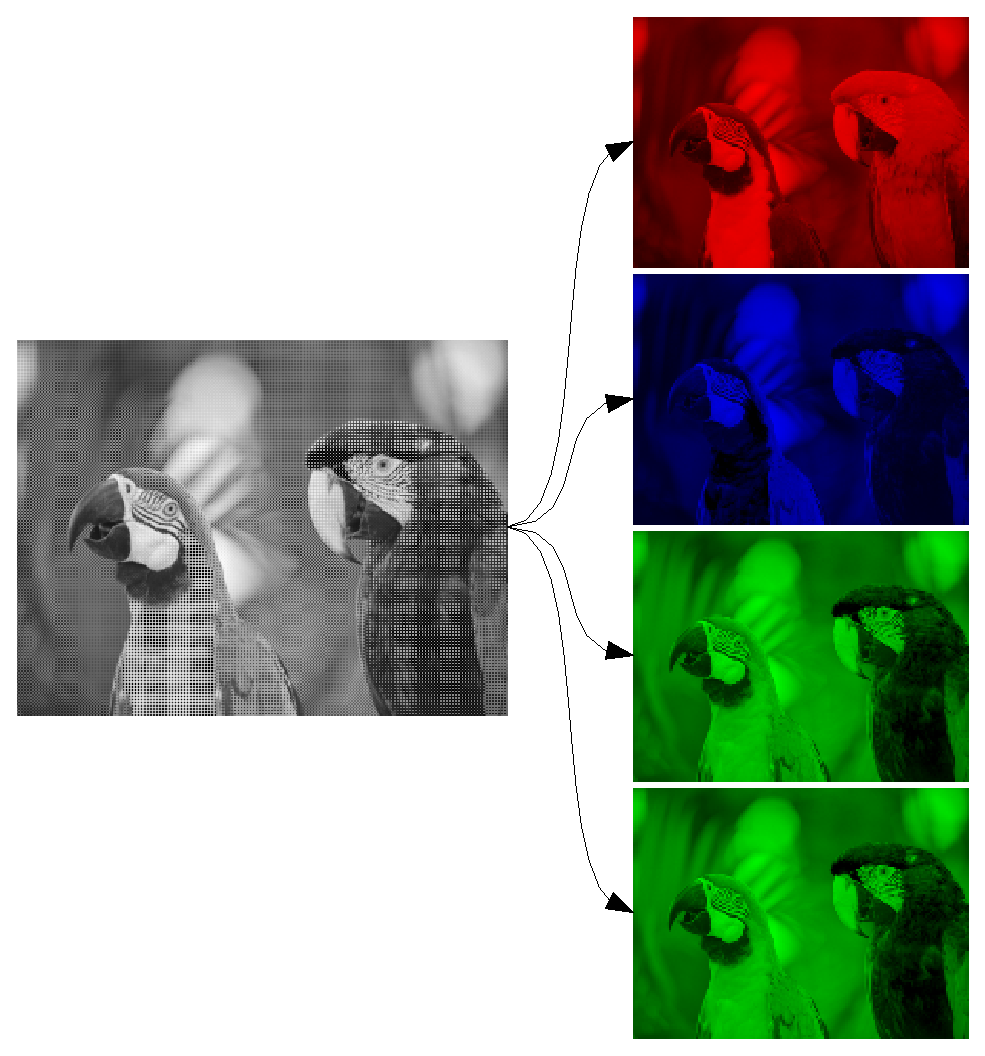
\includegraphics{channel_extraction}
\caption{Color channel extraction by texture minification.}
\label{fig:channel_extraction}
\end{figure}

\subsection{Interpolation and Blending}

The four color channel textures are rendered into another texture the
size of the original Bayer pattern texture.  By setting the texture
magnification function for each of the four color channel textures to
\texttt{GL\_LINEAR}, the missing pixels in each channel are bilinearly
interpolated from the available ones.

Multitexturing is used to render the four color channel textures into
the new texture, as seen in Figure~\ref{fig:interpolation}.  Each
color channel texture is bound to its own texture unit.  The two green
textures are blended into the new texture by using the
\texttt{GL\_ARB\_texture\_env\_combine} extension.  The red and blue
textures are then added to the composite texture by using the
\texttt{GL\_ARB\_texture\_env\_add} extension.

\begin{figure}
\centering
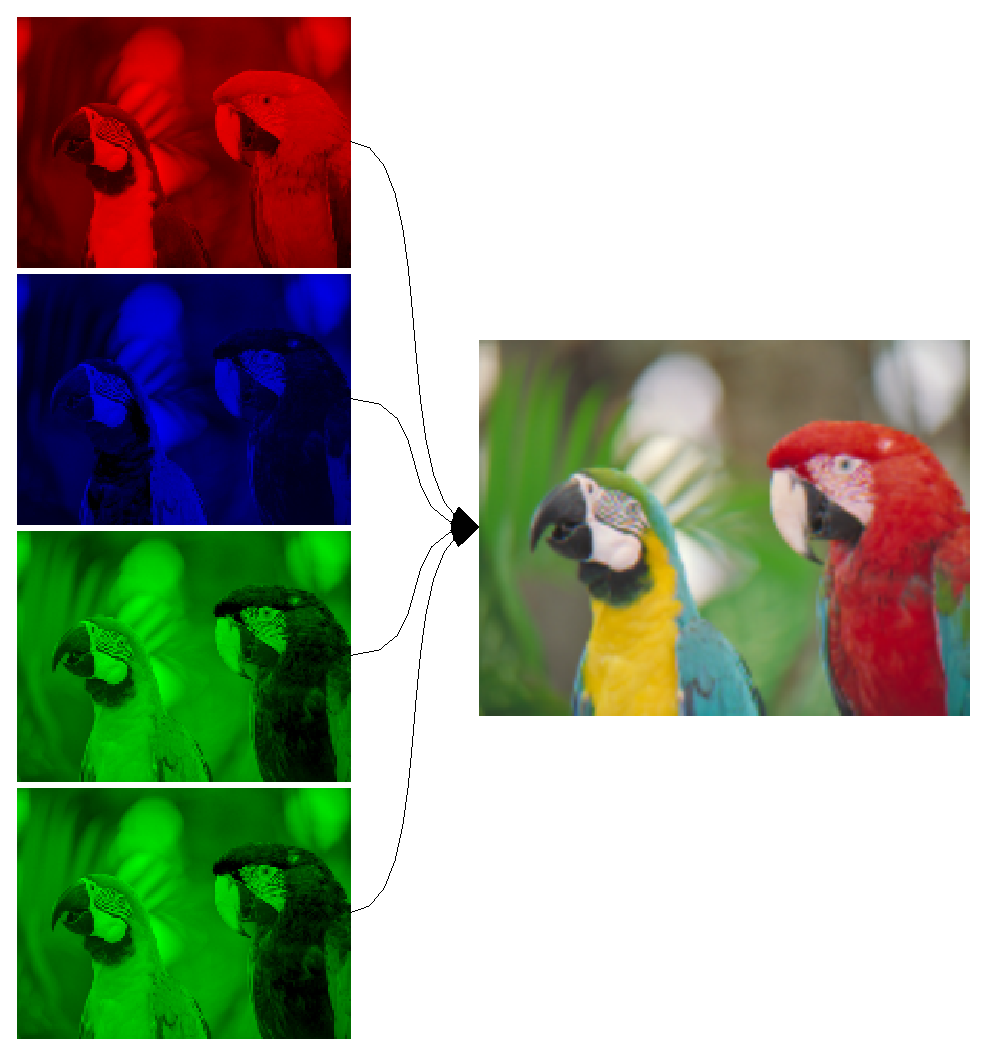
\includegraphics{interpolation}
\caption{The four color channel textures combine to form the RGB texture.}
\label{fig:interpolation}
\end{figure}
\section{Using the BayerRenderer Class}

The BayerRenderer header file must be included, and a
\texttt{BayerRenderer} object instantiated:
\begin{verbatim}
#include "BayerRenderer.hpp"

BayerRenderer br;
\end{verbatim}

Initialize the \texttt{BayerRenderer} once with the dimensions of the
Bayer pattern image:
\begin{verbatim}
br.Initialize (width, height);
\end{verbatim}

In the display loop, assuming \texttt{bayer} is a pointer to the Bayer
image data, the interpolated RGB image is bound to a texture with the
following code:
\begin{verbatim}
br.SetBayer (bayer);
br.Bind ();
br.EnableTextureTarget ();
// draw using decoded Bayer pattern image texture
br.DisableTextureTarget ();
\end{verbatim}

The Bayer pattern image should be stored as \texttt{GLubyte} data in
row-major order in a memory block of size \texttt{width * height}.
\section{Performance}

The OpenGL Bayer renderer gives about a four times speed improvement
compared to interpolating on the CPU.  On Linux, with a 640x480 image,
the CPU interpolation runs at approximately 50 fps, and the OpenGL
interpolation runs at approximately 200 fps.  The testing computer is
a 3.0~GHz Pentium~4 with an NVIDIA Quadro~FX~500 graphics card.

\bibliography{bayer_renderer}
\bibliographystyle{unsrtnat}
\end{document}

% LocalWords:  OpenGL's EnableTextureTarget GHz NVIDIA Quadro FX unsrtnat
